%!TEX program = xelatex
\documentclass{article}  
\usepackage[UTF8]{ctex} 
\usepackage{amsmath, amsthm, amssymb, graphicx}

\usepackage{minted} 
\usemintedstyle{xcode}
\usepackage{graphicx}

% Language setting
% Replace `english' with e.g. `spanish' to change the document language
\usepackage[english]{babel}

% Set page size and margins
% Replace `letterpaper' with `a4paper' for UK/EU standard size
\usepackage[letterpaper,top=2cm,bottom=2cm,left=3cm,right=3cm,marginparwidth=1.75cm]{geometry}

% Useful packages
\usepackage[colorlinks=true, allcolors=blue]{hyperref}

\title{Xunzhe Zhou's Homework 1}
\author{Xunzhe Zhou}

\begin{document}
\maketitle

\begin{abstract}
This file is the first homework of Python Programming Homework taught by Prof. Chen, Wenbin. This homework contains overleaf demos, ta-lib installation, proof of Riemann Hypothesis, odds calculation implemented by Python.
\end{abstract}

\section{Attempt of using TA-LIB}

This is a Python wrapper for \href{http://ta-lib.org}{TA-LIB} based on Cython
instead of SWIG. From the homepage:

TA-Lib is widely used by trading software developers requiring to perform technical analysis of financial market data. Includes 150+ indicators such as ADX, MACD, RSI, Stochastic, Bollinger Bands, etc. Candlestick pattern recognition. Open-source API for C/C++, Java, Perl, Python and 100\% Managed .NET.

\subsection{Installation}

\begin{minted}[mathescape,
    linenos,
    numbersep=5pt,
    gobble=2,
    frame=lines,
    framesep=2mm]{python}
    $ python -m pip install TA-Lib
\end{minted}

\subsection{Function API}

Similar to TA-Lib, the Function API provides a lightweight wrapper of the
exposed TA-Lib indicators.

Each function returns an output array and have default values for their
parameters, unless specified as keyword arguments. Typically, these functions
will have an initial "lookback" period (a required number of observations
before an output is generated) set to "NaN".

For convenience, the Function API supports both "numpy.ndarray" and
"pandas.Series" and "polars.Series" inputs.

All of the following examples use the Function API:

\begin{minted}[mathescape,
    linenos,
    numbersep=5pt,
    gobble=2,
    frame=lines,
    framesep=2mm]{python}
    import numpy as np
    import talib
    
    close = np.random.random(100)
\end{minted}

\section{Some examples to get started}

\subsection{Proof of Riemann Hypothesis}

The Riemann Hypothesis states that all non-trivial zeros of the Riemann zeta function have their real part equal to $1/2$. The Riemann zeta function is defined as:

\[
\zeta(s) = \sum_{n=1}^{\infty} \frac{1}{n^s} ,
\]

where $s$ is a complex number, and the series converges when the real part of $s$ is greater than $1$.

\subsection{How to add Pictures}

\begin{figure}[htbp]
\centering
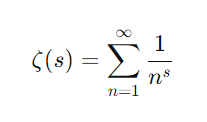
\includegraphics[width=0.25\linewidth]{Riemann.png}
\caption{\label{fig:Riemann}This picture is a screenshot of Riemann Hypothesis.}
\end{figure}

\subsection{How to add Tables}

Use the table and tabular environments for basic tables --- see Table~\ref{tab:widgets}, for example. For more information, please see this help article on \href{https://www.overleaf.com/learn/latex/tables}{tables}. 

\begin{table}
\centering
\begin{tabular}{l|r}
Item & Quantity \\\hline
Widgets & 42 \\
Gadgets & 13
\end{tabular}
\caption{\label{tab:widgets}An example table.}
\end{table} 

\subsection{How to add Lists}

You can make lists with automatic numbering \dots

\begin{enumerate}
\item Like this,
\item and like this.
\end{enumerate}
\dots or bullet points \dots
\begin{itemize}
\item Like this,
\item and like this.
\end{itemize}

\subsection{How to change the language of the document}

Overleaf 支持多种不同的语言,包括一份文档中的多种不同语言。

要配置文档语言,只需编辑此示例项目顶部序言中提供给 babel 包的选项即可。 要了解有关不同选项的更多信息,请访问\href{https://www.overleaf.com/learn/latex/International_language_support}{international language support}上的帮助文章。

要更改拼写检查语言,只需打开编辑器窗口左上角的 Overleaf 菜单,向下滚动到拼写检查设置,然后进行相应调整。

\subsection{How to add Citations and a References List}

You can simply upload a \verb|.bib| file containing your BibTeX entries, created with a tool such as JabRef. You can then cite entries from it, like this: \cite{zhouxunzhe}. Just remember to specify a bibliography style, as well as the filename of the \verb|.bib|. You can find a \href{https://www.overleaf.com/help/97-how-to-include-a-bibliography-using-bibtex}{video tutorial here} to learn more about BibTeX.

If you have an \href{https://www.overleaf.com/user/subscription/plans}{upgraded account}, you can also import your Mendeley or Zotero library directly as a \verb|.bib| file, via the upload menu in the file-tree.

\bibliographystyle{alpha}
\bibliography{sample}

\end{document}